\documentclass[conference]{IEEEtran}
\IEEEoverridecommandlockouts
% The preceding line is only needed to identify funding in the first footnote. If that is unneeded, please comment it out.
\usepackage{cite}
\usepackage{minted}
\usepackage{amsmath,amssymb,amsfonts}
\usepackage{algorithmic}
\usepackage{graphicx}
\usepackage{textcomp}
\usepackage{xcolor}
\usepackage{hyperref}
\usepackage[utf8]{inputenc}
\usepackage[spanish]{babel}
\def\BibTeX{{\rm B\kern-.05em{\sc i\kern-.025em b}\kern-.08em
    T\kern-.1667em\lower.7ex\hbox{E}\kern-.125emX}}
\begin{document}

\title{Optimización de ataques sobre CAPTCHA usando HPC\\
}

\author{\IEEEauthorblockN{1\textsuperscript{st} Gonzalo Larghero Valdivia}
\IEEEauthorblockA{\textit{Estudiante de grado Ingenieria en Computación} \\
\textit{Universidad de la República}\\
Montevideo, Uruguay \\
gonlarghero@gmail.com}
\and
\IEEEauthorblockN{2\textsuperscript{nd} Nicolas Izquierdo Signorelli}
\IEEEauthorblockA{\textit{Estudiante de grado Ingenieria en Computacion} \\
\textit{Universidad de la República}\\
Montevideo, Uruguay \\
nicoizquierdo95@gmail.com}}

\maketitle

\begin{abstract}
Dentro de los métodos de cracking de contraseñas los ataques de fuerza bruta (en los que se prueban todas las combinaciones posibles hasta encontrar aquella que permite el acceso) son de los mas sencillos y a la vez los mas costosos computacionalmente. 
Los factores determinantes en el coste de realizar un ataque de fuerza bruta son el largo de la clave y el conjunto de caracteres que se pueden utilizar en la clave, teniendo el aumento del largo de la clave una mayor influencia. Por ejemplo si se consideran estas dos contraseñas: \textit{madfapdfecabhdratreq} y \textit{Ga!9z3rm@u\&6}, la primera (a pesar de estar construida a partir de un conjunto mas pequeño de caracteres) es mas costosa de generar que la segunda debido a la cantidad de diferentes combinaciones que se obtienen usando una contraseña mas larga. La fuerza bruta suele combinarse con ataques de diccionario, estos tipos de ataques consisten en intentar averiguar una contraseña probando todas las palabras de una lista o 'diccionario'. Estos tipos de ataques, no son rápidos, para una contraseña compleja, puede llegar a tardar siglos. Es por eso que el presente trabajo se enfoca en aplicar las ventajas del procesamiento en paralelo con el objetivo de optimizar estos ataques sobre un captcha.
\newline
\end{abstract}

\begin{IEEEkeywords}
fuerza bruta, captcha, ataques diccionario, password cracking, paralelismo
\end{IEEEkeywords}

\section{Introducción}
Captcha o CAPTCHA son las siglas de Completely Automated Public Turing test to tell Computers and Humans Apart (prueba de Turing completamente automática y pública para diferenciar ordenadores de humanos). El test de Turing (o prueba de Turing) es una prueba creada con la intención de medir que tan cercano al comportamiento de un humano es el comportamiento inteligente de una máquina. Aunque el test de Turing es controlado por un humano los captchas son controlados por una máquina, por ello, consiste en una prueba de Turing inversa. Normalmente se trata de una prueba desafío-respuesta utilizada en computación para determinar cuándo el usuario es o no humano. El término se empezó a utilizar en el año 2000 por el guatemalteco Luis von Ahn (fundador de las compañías Duolingo, Captcha y Recaptcha) y fue popularizado por  Manuel Blum y Nicholas J. Hopper de la Universidad Carnegie Mellon, junto a John Langford de IBM. El formato de captcha mas popular consiste en que el usuario introduzca correctamente un conjunto de caracteres que se muestran en una imagen distorsionada que aparece en pantalla suponiendo que una máquina no es capaz de comprender e introducir la secuencia de forma correcta, por lo que solamente un humano podría hacerlo. \newline \\
Los captchas son utilizados para evitar que robots, también llamados spambots, puedan utilizar ciertos servicios. Por ejemplo, para privarlos de participar en encuestas o foros de discusión, registrarse para usar cuentas de correo electrónico y recientemente, para evitar que un bot de este tipo pueda enviar correo basura (el remitente debe pasar el test antes de que se entregue al destinatario).\newline \\
La mayoría de los captchas utilizan desafíos relacionados con el reconocimiento de texto en el formato de imagen, al que se le agrega distorsión con el objetivo de evitar el software de OCR (Optic Character Recognition). Normalmente se introduce algún tipo de 'ruido de fondo' generado pseudo-aleatoriamente en la imagen, esto permite ver al captcha como una especie de cifrado, similar a un Hash en el cual se parte de un texto y se genera un resultado cifrado. Por supuesto que para un humano sería fácil de descifrar utilizando una interpretación visual, pero para una maquina no es tan sencillo obtener un texto a partir de un conjunto de píxeles. Es por esto que la aplicación de ataques de diccionario o fuerza bruta sobre los captchas es especialmente difícil. No solo requiere tener acceso a la función de generación de captcha, también requiere utilizar todas las combinaciones de ruido de fondo utilizadas en el generador para cada palabra que se va a testear. La utilización de OCR es un enfoque mucho mas practico a este problema intentando simular la interpretación visual que haría un humano, pero estas tecnologías no están completamente maduras y tienen grandes dificultades especialmente contra captchas, los cuales como ya se dijo son especialmente diseñados para ser difíciles de reconocer. En este caso el hecho de que, en un ataque diccionario,se deban generar una gran cantidad de imágenes (utilizando toda las combinaciones de palabras y ruido de fondo) y que sean todas las generaciones independientes entre si nos permite sacar mayor provecho del procesamiento en paralelo, como se demuestra a continuación.

\section{Descripción del problema}

El problema a desarrollar consiste en implementar un programa que permita dado un captcha generado (a través de una metodología conocida) utilizar los beneficios de la programación paralela para obtener la palabra que fue usada para generar la imagen (al igual que si la generación de la imagen fuera una forma de encriptación del texto).

\begin{figure}[h]
  \centering
   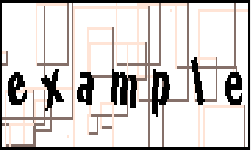
\includegraphics[width=0.3\textwidth]{Captura.PNG}
 \end{figure}

Para este proyecto se adaptó el código de generación de captchas obtenido en \href{https://javadiscover.blogspot.com/2013/07/creating-captcha-using-java.html}{este sitio}\cite{b1} debido a que permite control total sobre las variables responsables de la generación de ruido de fondo. Entre las modificaciones realizadas se incluyen disminuir los espacios utilizados para generar las figuras usadas como ruido de fondo, los ángulos de las letras y la elección del texto en si. Esto se debe a que era necesario disminuir la escala del problema para poder obtener resultados a corto plazo durante la etapa de desarrollo, disminuyendo la complejidad sin alterar el funcionamiento. Si se dispusiera de una cantidad de tiempo suficiente o más recurso de cómputo, se podría aumentar la complejidad de la generación de captcha.  Para el caso de los ángulos se limitó a nueve posibles ángulos para cada letra, para el texto se seleccionaron las palabras de un diccionario (para eliminar la elección aleatoria de cada letra) y para el caso de las figuras de fondo se generaron una gran cantidad de patrones aleatorios y luego se hizo que los captchas eligieran entre los patrones generados en vez de generar uno nuevo cada vez. De esta forma de mantuvieron las elecciones aleatorias de palabra, ángulos e imágenes de fondo, pero se redujeron las combinaciones posibles para de-escalar el problema. Como era de nuestro interés realizar ataques de fuerza bruta se agrego una funcionalidad para permitir la generación de captchas a partir de texto ingresado por el usuario de forma que no todos los captchas generador pudieran ser atacados mediante ataques diccionario.\newline En resumen se implementa un programa que ataca a la imagen generada en dos fases (primero utilizando un diccionario y luego fuerza bruta) teniendo en cuenta que para cada texto se deben comparar todos los ángulos posibles y todas las posibles combinaciones de imágenes de fondo.

\section{Utilización de HPC}
Como ya se mencionó anteriormente la implementación de ataques diccionario requiere la utilización de una función de encriptado (en este caso la generación del captcha) y luego la comparación para cada palabra en el diccionario, mientras que las de fuerza bruta realizan lo mismo con todas las palabras posibles (dado el largo n a intentar) dado un alfabeto conocido. Para hacer un buen uso del procesamiento en paralelo se debe tener en claro qué parte del proceso es la más \textit{CPU-intensive} ya que esa es la sección de trabajo que dará mas beneficios al ser distribuida. En un ataque de diccionario normal, obtener los hashes para cada palabra tiene un uso mayor del procesador que la comparación de strings pero para el caso de este proyecto no es tan evidente. En este caso, la comparación de imágenes es mucho mas compleja que la comparación de strings, también la generación de captchas puede variar enormemente en complejidad. Para resolver este problema se decidió repartir tanto la generación como la comparación entre los múltiples threads ya que esto no estaba previsto dentro de los objetivos de este proyecto. Sin embargo en caso de que interese resolver esta duda se podría separar el trabajo en dos threads (uno que genere los captchas y otro que los compare) de forma que sea mas fácil evaluar cual es el cuello de botella y por lo tanto la parte más \textit{CPU-intensive}. Cabe agregar que este modelo requeriría más comunicación entre threads así que incluso si una de las dos tareas (generación y comparación) es mas intensa que la otra el mantenerlas en un bloque de trabajo dentro de un thread tiene sus ventajas.\newline

Dicho esto se separó el trabajo en bloques de palabras de largo fijo. Es fácil darse cuenta que cada bloque es independiente de los demás por lo que es un candidato perfecto para las técnicas de paralelización de HPC. 
Es por esto que la técnica de paralelización usada consiste en dividir el conjunto de palabras utilizadas en el ataque (ya sea un diccionario o la totalidad de palabras posibles en el caso de fuerza bruta) en bloques y realizar todo el proceso de generación de todos los posibles captchas y sus comparaciones de forma paralela.
Este modelo además tiene la ventaja de que no se requiere comunicación extra entre threads salvando la excepción de que un thread haya encontrado la palabra que generó la imagen. Gracias a esto se debería reducir el tiempo de calculo considerablemente.

\section{Estrategia de paralelización}
Teniendo en cuenta los puntos destacados anteriormente se diseñó una solución al problema utilizando el lenguaje de programación java y sus herramientas de programación para multithreading: \textbf{runnable}\cite{b3} y \textbf{callable} \cite{b4}. Java provee varias ventajas, en comparación con los lenguajes utilizados en el curso, no solo en términos de interfaz sino también para el manejo de imágenes y su comparación. Esta claro que nada de lo realizado en este proyecto está atado al lenguaje utilizado y puede ser replicado en C, C++ o cualquier lenguaje que soporte manejo de threads de ser necesario. \newline

\begin{figure}[h]
  \centering
   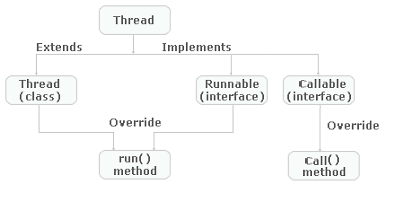
\includegraphics[width=0.5\textwidth]{Captura2.png}
 \end{figure}

Las herramientas nombradas previamente son interfaces previstas por java para el trabajo en programación concurrente y por lo tanto ambas clases podrían verse como extensiones de la clase \textbf{Thread} pero hay que aclarar que tienen diferencias. Usualmente se recomienda evitar la clase Thread completamente ya que en la mayoría de los casos de Multithreading (este incluido) la vida del thread está relacionada a cierta tarea y por lo tanto no se necesita tanto control sobre el comportamiento del thread en si. Por lo tanto implementar las clases Runnable y Callable permite usar threads relacionados solamente a una simple función a implementar (run o call respectivamente) y desligarnos de los problemas de especificar el comportamiento del thread (de la misma forma que utilizando al librería pthread.h en C para llamar los threads a una función).
La diferencia entre ambas es que la función run es de tipo void y por lo tanto si se quisiera guardar resultado alguno, se tendrá que utilizar una variable compartida global. La interfaz callable por el otro lado puede tener un retorno de cualquier tipo (llamemosle T) y nos permite llamarla de la forma
\begin{minted}[escapeinside=||,mathescape=true]{java}
Future<T> return = Class.call();
\end{minted}
donde el wrapper future nos permite saber el estado del thread (si terminó o no de realizar la tarea dentro del call). 

\subsection{Generación del captcha}
La generación de los captchas se implementó en tres modalidades:
\begin{enumerate}
   \item Selección aleatoria acotada (seleccionando el texto  aleatoriamente desde un diccionario predefinido, y generando ángulos y figuras aleatorias)
    \item Texto dado (tomando el texto  pasado como parámetro y generando ángulos y figuras aleatorias)
    \item Fijo (Tomando todos las variables posibles por parámetro o archivo de configuración)
\end{enumerate}
El primer caso permite generar captchas aleatorios que puedan ser objetivo de ataque diccionario. El segundo caso permite generar captchas que se puedan usar para probar fuerza bruta. Y finalmente el tercer caso permite a los threads generar captchas para comparar con la víctima. Los parámetros que se pasan en el tercer caso incluyen texto, ángulo de cada letra y posición de los artefactos colocados como ruido de fondo.\newline
Ignorando de momento el texto utilizado para el captcha, ya que los valores a tomar varían dependiendo de si se usa un ataque diccionario o fuerza bruta, los ángulos tienen nueve posibles valores y los artefactos de fondo tienen cien combinaciones posibles. Sin embargo es evidente que mientras la cantidad de artefactos de fondo es constante y por lo tanto siempre se generarán cien posibles captchas por cada texto, el ángulo de las letras aumenta exponencialmente la cantidad de capachas a medida que la cantidad de letras en el texto aumenta.
Esto queda más claro en la siguiente formula:
\[PC = 100 *\sum_{i = 0}^{i = P-1} 9^{L_i}\]
donde: 
\begin{itemize}
    \item PC = cantidad de Posibles Captchas
    \item P = cantidad de Palabras
    \item $L_i$ = cantidad de Letras de cada palabra
\end{itemize}
Por ejemplo si todas las palabras tuvieran seis letras se podrían generar 53.144.100 posibles combinaciones de captcha para cada palabra, y hay 387.420.489 posibles palabras lo cual deja un total de $2.05 * 10 ^{16}$ combinaciones. Se debe tomar en cuenta que estas operaciones no son sencillas, es decir que no se ejecutan en el procesador como una única operación, por lo que se puede esperar un alto costo computacional. Si se utilizan todas las palabras de largo cuatro se obtienen 348.678.440.100 las cuales implican aproximadamente 60.000 veces menos operaciones, una cantidad mas accesible para las pc de escritorio actuales. Es por esto que no se utilizaran palabras de mayor largo para la toma de datos experimentales en este proyecto. Esto aplica a la mayoría de las variables utilizadas, la generación de capchas habilita una gran cantidad de parámetros en espacios densos por lo que en teoría se podrían generar infinitas combinaciones de ángulos y artefactos, sin embargo aquí se usan cantidades limitadas y todo puede escalarse en caso necesario.
\subsection{Comparación del resultado}
En el momento en que cada thread genera una imagen, esta se compara con la imagen objetivo. Se implementó una función que en principio compara los tamaños de las imágenes y luego itera sobre los píxeles de estas. En caso de que cada uno de los píxeles sean iguales, el comparador devuelve como positiva la comparación. El comparador devuelve negativo en cualquier otro caso. Cabe destacar que cuando un thread obtiene una imagen igual a la imagen objetivo, se notifica al resto de los threads mediante el uso de una variable global, para evitar uso adicional de recursos.. 
\subsection{Arquitectura de la solución}

Con el objetivo de poder comparar los resultados de diferentes tipos de ataques y obtener conclusiones más claras se desarrollaron múltiples versiones de algoritmo.\newline
Dependiendo de los parámetros de entrada seleccionados se 
cuenta con un algoritmo con balance de carga estático y otro dinámico, se puede variar si se desea trabajar con fuerza bruta o ataque diccionario e incluso la cantidad de threads a utilizar.
El programa cuenta con cuatro módulos principales, uno que controla los parámetros y el loop sobre las pruebas que se realizarán, un datatype que contiene todos los datos necesarios para una ejecución concreta, un módulo encargado de la ejecución del ataque y por ultimo el generador de captchas. 
El programa contaba previamente con una interfaz gráfica que mostraba el captcha generado y permitía el ingreso de forma sencilla de la palabra a utilizar para su generación, esta parte del programa fue eliminada debido a la necesidad de ejecutar nuestro código desde consola (dentro del cluster).


\subsection{Balance de carga}
Se evaluaron diversas implementaciones del balance de cargas, finalmente se optó por implementarlo usando colas de trabajo dinámicas. Cada thread cuenta con su propia cola de trabajo en la cual se almacenan los bloques de palabras que cada thread deberá procesar.\newline Cuando comienza la ejecución del ataque, ya sea fuerza bruta o de diccionario, se agrupa el conjunto total de palabras en bloques de trabajo y estos se dividen en un numero definido previamente de subconjuntos de igual cantidad de elementos. Como primer paso se distribuyen los bloques del primer subconjunto de forma equitativa entre las colas de trabajo de cada thread. Cuando un thread finaliza el procesamiento de su respectiva cola de trabajo, se distribuye otro subconjunto de bloques en las colas de trabajo. Sin embargo esta vez no es de forma equitativa, sino proporcional a la cantidad de bloques procesados. Es decir que cada thread obtendrá una cantidad de trabajo acorde a la velocidad de procesamiento que tuvo hasta el momento. \newline

Cabe destacar que esta distribución asocia velocidad de procesamiento con cantidad de bloques procesados. Esta afirmación solo puede ser correcta si los bloques distribuidos en las colas de trabajo tienen un tiempo similar de procesamiento, lo cual se trató de lograr ordenando el diccionario por largo de palabra y no de forma alfabética. Un posible problema surge si un thread comienza trabajando a mayor velocidad que los demás pero se  vuelve mas lento con el pasar del tiempo, aun seguirá recibiendo una mayor proporción de bloques debido a su buena performance durante las primeras iteraciones. Como solución se calcula el rendimiento de un thread basándose solamente en los bloques de trabajo procesados durante el subconjunto anterior. \newline

Luego de terminar la distribución de todos los bloques de trabajo, si un thread vacía su cola, este comenzará a tomar bloques de trabajo de la cola con más elementos en ese momento. Nuevamente este no tomará una cantidad fija de elementos, sino que tomará una cantidad proporcional a su cantidad de bloques procesados. \newline
El programa desarrollado tiene la opción de deshabilitar el balance de cargas, el comportamiento obtenido al hacerlo consiste en dividir el total de bloques de palabras equitativamente entre todos los threads. Cuando uno termine de procesar los bloques que le correspondan simplemente se liberará la memoria asignada, eliminando así el thread en cuestión.

\subsection{Tolerancia a fallos}
La tolerancia a fallos es un tema complejo de manejar en la programación multithreading por lo cual se intentó implementarlo de la forma mas simple posible sin perder los beneficios de tolerar errores. Si en algún momento un thread dispara una excepción, esta es capturada. Se libera el thread que obtuvo la excepción y se ejecuta una función estática que genera un nuevo thread. A este nuevo threads se le asigna la cola de trabajo del thread que disparó la excepción. En esta cola de trabajo está incluido el bloque que estaba procesando el thread fallido previamente. La ventaja de la implementación realizada es que no se desaprovechan los bloques que se procesaron totalmente. La desventaja es que si la excepción se disparó por problemas en los datos, el nuevo thread generado también arrojará la misma excepción. Una solución posible sería descartar los bloques que generen errores en su procesamiento, identificando el error en los datos mediante el fallo reiterado. De todas formas durante la realización de pruebas quedo claro que los casos de error eran mínimos y no afectaban el funcionamiento normal del programa.

\section{Evaluación experimental}
\subsection{Primer intento de evaluación}
En nuestro primer intento de evaluación experimental se realizaron distintas pruebas de la implementación variando factores clave tales como la cantidad de threads, la distribución de bloques de trabajo, el largo de palabra y el método de ataque (diccionario y fuerza bruta).

Las pruebas se realizaron en un nodo del cluster de facultad, el cual cuenta con un cpu Xeon Gold 6138 de 20 núcleos y 40 threads con una frecuencia de 2.00 GHz y una frecuencia en turbo de 3.70 GHz máximo \footnote{https://ark.intel.com/content/www/es/es/ark/products/120476/intel-xeon-gold-6138-processor-27-5m-cache-2-00-ghz.html}. Por temas de tiempo se optó por tomar mediciones de 1, 4, 8, 16 y 32 threads.

Hay que tener en cuenta que para este tipo de carga altamente paralelizable la cantidad de threads es mucho mas importante que la velocidad de los mismos por lo que no habría mucha diferencia al utilizar una pc de escritorio con la misma cantidad de threads.  Se decidió no considerar las palabras cuyo largo superara las 5 palabras debido a la gran cantidad de tiempo que se le debería dedicar para tomar datos concluyentes.\newline
Cada ataque de diccionario utilizó quinientas palabras distintas en total. Número elegido para mantener los tiempos no demasiado altos, pero con la cantidad de palabras suficientes como para apreciar cambios en los tiempos de ejecución al variar parámetros. El ataque de fuerza bruta utiliza todo el conjunto de palabras posibles generadas a partir del alfabeto. \newline

Por último para asegurar que cada una de las ejecuciones procesara el total de palabras disponibles, se generó un captcha con una palabra que poseyera una letra no incluida en el alfabeto. Esta medida fue tomada ya que según la distribución estática o dinámica, se podría dar que los tiempos para encontrar la palabra correcta varíen de forma impredecible. Es decir que una distribución podría ser más rápida que otra simplemente porque encontró la palabra correcta antes, y no por procesar bloques de trabajo en menos tiempo.\newline

Este método de evaluación se topa rápidamente con un problema de escala, los ataques de fuerza bruta son ciertamente viables para palabras de tres letras de largo pero teniendo en cuenta un alfabeto de 26 caracteres la cantidad de tiempo requerido para las pruebas se escapa de lo disponible para este proyecto. 

\subsection{Segunda metodología de evaluación}

Al medir la eficiencia del uso de multi-threading para lidiar con el problema planteado no hace diferencia si se esta atacando una lista de palabras pertenecientes a un diccionario o a una lista de palabras completa generada para un ataque de fuerza bruta, por lo tanto como primera mejora se eliminó esta variable de nuestra evaluación, dejando así una única lista de palabras correspondiente al conjunto de palabras posibles generadas a partir del alfabeto. 
Como segunda mejora se realizaron dos pruebas por separado una para comparar los cambios de performance al aumentar la cantidad de threads y otra para comparar la distribución de carga estática contra la dinámica ya que aislar las variables permite un mejor entendimiento de los resultados.
Como tercer mejora se realizaron las pruebas en tres sistemas distintos, no solo el cluster ya mencionado sino también en sistema de escritorio y en un servidor. El sistema de escritorio esta equipado con un procesador AMD Ryzen 5 3600 de 6 núcleos y 12 threads con una frecuencia de 3.6 GHz y una velocidad de hasta 4.2 GHz de turbo \cite{b7} mientras que el servidor esta equipado con un procesador Xeon Gold 5220 de 14 núcleos y 28 threads con una velocidad base de 2.2 GHz y un turbo de 3.2 GHz \cite{b8}.
Por último para asegurar que los resultados terminen en un tiempo razonable las pruebas sobra la variable de cantidad de threads miden la cantidad de palabras procesadas en un tiempo fijo y no al revés como en la metodología inicial. Todas las pruebas se realizaron dos veces para evitar anomalías, los resultados mostrados a continuación son promedios.

\begin{figure}[h]
  \centering
   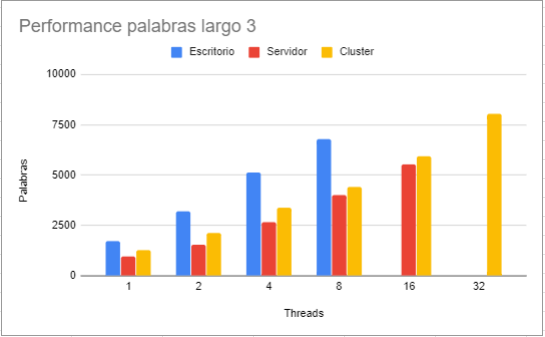
\includegraphics[width=0.5\textwidth]{Captura3.PNG}
 \end{figure}

\begin{figure}[h]
  \centering
   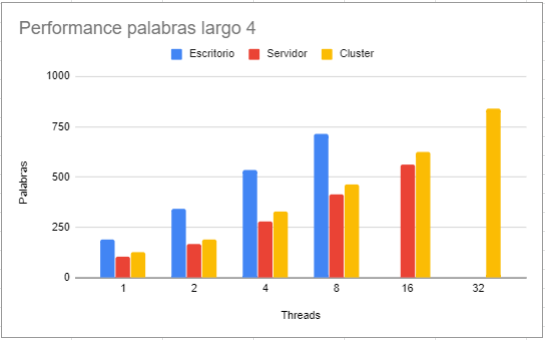
\includegraphics[width=0.5\textwidth]{Captura5.PNG}
 \end{figure}

\begin{figure}[h]
  \centering
   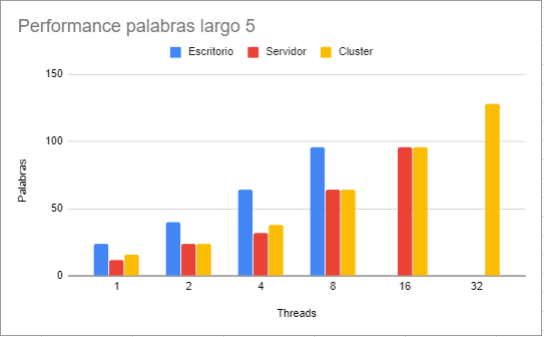
\includegraphics[width=0.5\textwidth]{Captura4.PNG}
 \end{figure}

\newpage

\subsubsection{Distribución estática vs Dinámica}

Al comparar la distribución estática contra la dinámica en cuanto a tiempos se obtuvieron peores resultados utilizando la distribución dinámica. Esto dos razones principales, la primera y más importante es que los threads no tienen una gran diferencia en performance entre si como se muestra en el gráfico a continuación.

\begin{figure}[h]
  \centering
   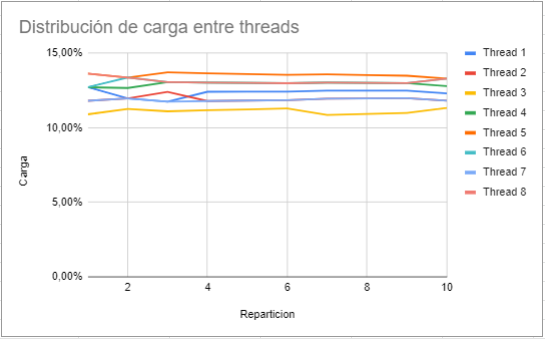
\includegraphics[width=0.5\textwidth]{Captura6.PNG}
 \end{figure}

Debido a esto el redistribuir la carga múltiples veces (lo cual implica una posible parada a todos los threads mientras se modifican sus colas de trabajo)\footnote{No es seguro ya que si el thread se encuentra trabajando y en una palabra no lo afectara que su cola este detenida hasta haya terminado con su bloque de trabajo} solo sirve para ralentizar el proceso. 
La segunda razón y las más difícil de predecir es la distribución de la carga al momento de entrar en la etapa de \textit{robo} (cuando un thread vació su cola de trabajo y no quedan mas reparticiones, por lo que tiene que tomar de las de otros). El procedimiento de tomar una parte proporcional a la velocidad del thread que roba de la cola del thread con mas trabajo pendiente resulta contraproducente si todos los threads trabajan a casi la misma velocidad y tienen casi la misma cantidad de trabajo en cola. Se comienzan a producir una gran cantidad de interrupciones "robándose" entre ellos pequeñas porciones de trabajo (ya que proporcionalmente todos trabajan a la misma velocidad) sin tomar en cuenta que el thread con mas trabajo en cola puede que no sea el objetivo correcto a robar. Una posible mejora sería robar no al que tenga más trabajo en cola sino al que tenga mayor ratio: \[\frac{trabajo}{velocidad}\] aunque aún en este caso la performance se vería afectada cuanto más baja sea la diferencia de velocidad entre los threads. La mejor forma de eliminar esta problema de robos continuos al final es limitar la cantidad de robos por thread, permitir una cantidad de uno o dos robos por thread.

\section{Conclusiones}
A continuación se comentaran las conclusiones que se obtuvieron en el desarrollo del proyecto a partir de los datos obtenidos.
En nuestra primera aproximación nos topamos con un problema de escalabilidad en el cual aumentar el tamaño de palabra, los tiempos de ejecución del ataque de fuerza bruta crecían de forma exponencial. Si bien probar todas las combinaciones de palabras de tres caracteres era posible, las combinaciones de cuatro y de cinco necesitaban una cantidad de tiempo muy superior. Debido a esto decidimos tomar un enfoque de velocidad de procesamiento de palabras por segundo, esto nos permitió hacer comparaciones de rendimiento en un tiempo razonable.
En nuestra segunda aproximación obtuvimos resultados verdaderamente interesantes, por un lado cabe destacar que al ejecutar en una maquina de escritorio usando un procesador con mas GHz de velocidad, esta fue mucho mas performante que el servidor y el cluster. Esto era esperable ya que en igual cantidad de threads, procesará más trabajo el que tenga mayor velocidad. Sin embargo al aumentar la cantidad de threads, tanto el cluster como el servidor aumentaron su rendimiento, alcanzando e incluso superando en varios casos a la maquina de escritorio, la cual contaba con un cpu mucho mas rápido. Esto lleva a la pregunta de ¿porque los cpu de servidores prefieren mantener velocidades bajas y aumentar la cantidad de núcleos? Hay varias razones pero la más importante es el control de temperatura, los servidores normalmente están pensados para procesamiento de gran cantidad de información por lo que se benefician de gran manera de tener muchos núcleos pero tener tantos núcleos a la misma velocidad de una maquina de escritorio traería mas complicaciones que beneficios. 
\begin{itemize}
    \item Altos costos en disipación de calor
    \item Altos costos en electricidad
    \item Requisitos mayores en cuanto espacio.
    \item Mayor inestabilidad, lo cual puede llevar a errores.
\end{itemize}
Las pruebas de cinco letras nos dejaron dos conclusiones interesantes, primero se puede ver que los resultados se ven más escalonados, esto se debe a que como las pruebas eran interrumpidas luego de cierto tiempo los threads tenían una mayor probabilidad de ser interrumpidos en el medio del procesamiento de un bloque por lo que ese trabajo se descartaba y se contaban solo los bloques procesados de forma completa. Y por otro lado estas pruebas aclaran la proporción de complejidad cuando se aumenta una letra en las palabras a procesar, disminuyendo a una decena por cada letra agregada.

Finalmente podemos concluir que el uso de threads para atacar este tipo de problemas es muy eficiente, ya que el aumento de la velocidad de procesamiento crecía casi lineal con respecto al número de threads. Además cabe destacar que para problemas como este, en los que se necesita ejecutar una misma tarea sobre una cantidad muy grande de datos, los threads son una herramienta que se debe tener en cuenta.  

\section{Trabajo a futuro}
Tomando todo lo dicho en las anteriores secciones, recopilamos las siguientes posibles mejoras que se pueden tener en cuenta para un trabajo a futuro:
\begin{itemize}
    \item Reducir el número de variables globales a la que acceden los threads ya que el acceso a memoria compartida afecta en cierta medida el rendimiento de estos.
    \item Probar distintos tamaños de bloques para el distinto largo de palabra y cantidad de estas. Puede que incrementar o disminuir el tamaño de los bloques en algunos casos m¿pueda mejorar el rendimiento, hasta se podría hacer en forma dinámica
    \item Una vez que un thread termine de procesar sus bloques elegir procesar los bloques del thread que trabaja más lento, y no del que tiene más trabajo. También limitar la cantidad de "robos" por unidad de tiempo ya que el exceso de estos puede degradar los tiempos de ejecución por el uso de recursos compartidos. 
\end{itemize}

\begin{thebibliography}{00}
\bibitem{b1} https://javadiscover.blogspot.com/2013/07/creating-captcha-using-java.html
\bibitem{b2} https://crambler.com/password-security-why-secure-passwords-need-length-over-complexity/
\bibitem{b3}https://docs.oracle.com/javase/7/docs/api/java/util/concurrent/Callable.html
\bibitem{b4} https://docs.oracle.com/javase/7/docs/api/java/lang/Runnable.html
\bibitem{b5} https://docs.oracle.com/javase/tutorial/uiswing/components/progress.html
\bibitem{b6} https://docs.oracle.com/javafx/2/api/javafx/concurrent/Task.html
\bibitem{b7} https://www.amd.com/es/products/cpu/amd-ryzen-5-3600
\bibitem{b8} https://ark.intel.com/content/www/us/en/ark/products/120474/intel-xeon-gold-5120-processor-19-25m-cache-2-20-ghz.html
\end{thebibliography}
\vspace{12pt}

\end{document}
